\begin{frame}
  \frametitle{El código de repetición en cuántica también funciona}
  \begin{columns}
    \begin{column}{0.45\textwidth}
      \begin{figure}[!htbp]
        \centering
        \begin{quantikz}
          \lstick{$\ket{\psi}$} & \ctrl{1} & \ctrl{2} & \qw \\
          \lstick{$\ket{0}$}     & \targ{}  & \qw      & \qw \\
          \lstick{$\ket{0}$}     & \qw      & \targ{}  & \qw
        \end{quantikz}
        \label{quantum_repetition_code_encode_circuit}
      \end{figure}
      \begin{figure}[H]
        \centering
        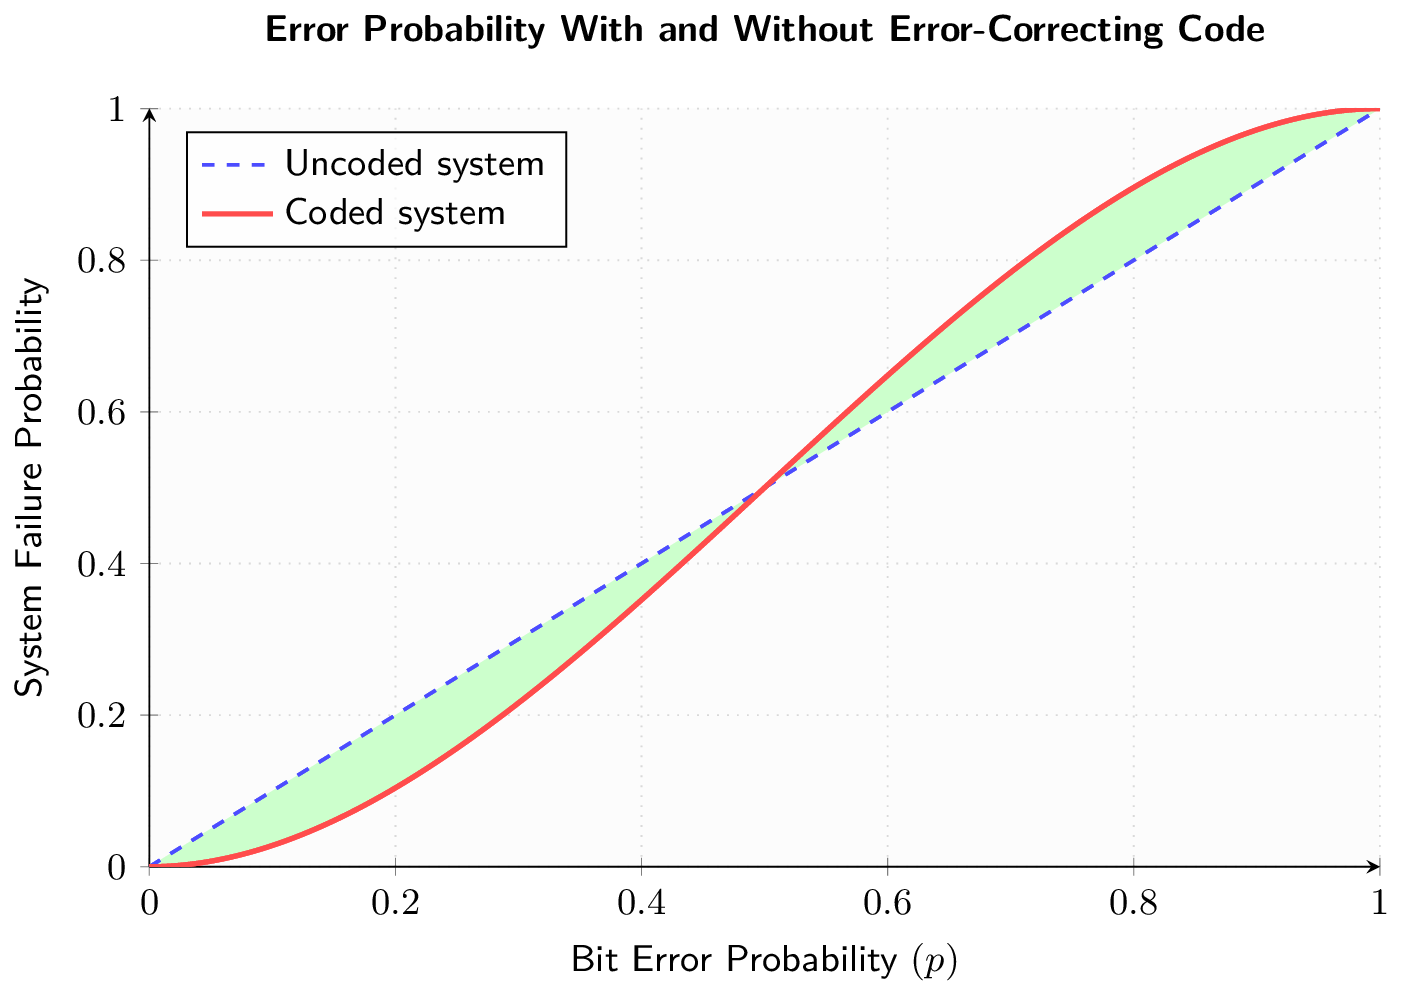
\includegraphics[width=0.7\linewidth]{files/02_comparison-2d9e0d455373d64bb1d46105fb84b631.png}
        \label{img_2}
      \end{figure}
    \end{column}
    \begin{column}{0.45\textwidth}
      Del mismo modo que en computación clásica, podemos codificar un qubit con \citep{Nielsen2010}:
      \begin{equation}
        \ket{0}_L = \ket{000};\quad \ket{1}_L = \ket{111}
        \label{eq:cod_repetition}
      \end{equation}

      Al codificar así, se tiene una fidelidad de \citep{Nielsen2010}:
      \begin{equation}
        p^3 + 3p^2(1 - p) = 3p^2 - 2p^3
      .\end{equation}

      Pero, como consideración, no corrige un error arbitrario; por ejemplo, para una codificación en la base canónica no corrige \textit{phase-flips}.
    \end{column}
  \end{columns}
\end{frame}
